\section{Post Processing}

	This section documents the path processing steps followed in this paper. The
	algorithm developed first tries to simplify the path by removing unnecessary
	intermediate poses and optimising the rotation trajectory. Next, it tries to
	locally optimise the capacity margin of the remaining poses and finally
	smoothly interpolates the path using B-splines.

	\subsection{Pose Removal}

		The path planning returns an ordered set of poses, $\setofposes$, such
		that, by connecting each pose with a straight line, the goal pose may be
		reached from the start pose without collisions. Due to the random nature
		of \gls{rrt}, however, there may be many unnecessary poses in
		$\setofposes$.

		Two simple algorithms are employed to remove unnecessary poses and
		shorten the total distance as measured by
		Equation~\ref{eq:distance_measure_capcity_margin}. These algorithms are
		described in the rest of this section.

		\subsubsection{Reducing Poses in $\setofposes$}

			The first algorithm simply removes a pose $\pose_i$ from
			$\setofposes$ if:

			\begin{itemize}

				\item

					Doing so decreases the total distance:

					\begin{equation}
						\dist(\pose_{i - 1}, \pose_{i + 1}) <
							\dist(\pose_{i - 1}, \pose_i)
							+ \dist(\pose_i, \pose_{i + 1})
					\end{equation}

				\item

					The straight-line path between $\pose_{i - 1}$ and $\pose_{i
					+ 1}$ is collision-free.

			\end{itemize}

			This algorithm is run recursively until no more poses can be
			removed.

		\subsubsection{Removing Corners from $\setofposes$}

			Consider three consecutive poses, $\pose_1, \pose_2, \pose_3 \in
			\setofposes$. After the pose removal step from before, it may happen
			that $\pose_2$ is fairly far from the rest of the path, but the
			straight line between $\pose_1$ and $\pose_3$ is not collision free.
			It is therefore desirable to find some pose $\pose_a$ on the line
			$\vecline{\pose_1}{\pose_2}$ and $\pose_b$ on
			$\vecline{\pose_2}{\pose_3}$ such that:

			\begin{equation}
				\dist(\pose_1,\pose_a) + \dist(\pose_a,\pose_b) +
				\dist(\pose_b,\pose_3)
				<
				\dist(\pose_1,\pose_2) + \dist(\pose_2,\pose_3)
			\end{equation}

			and such that the straight-line path between $\pose_a$ and $\pose_b$
			is collision-free.

			To find these poses such that:

			\begin{equation}
				(\pose_a, \pose_b) = \argmin
					(
						\dist(\pose_1, \pose_a) +
						\dist(\pose_a, \pose_b) +
						\dist(\pose_b, \pose_3)
					)
			\end{equation}

			the following parametric lines are used:

			\begin{align}
				\pose_a &= \pose_1 + \timenorm_a(\pose_2 - \pose_1)\\
				\pose_b &= \pose_3 + \timenorm_b(\pose_2 - \pose_3)
			\end{align}

			Then a simple two-dimensional binary search is performed on
			\(
				\timenorm_a, \timenorm_b \in [0, 1]
			\)
			in order to solve for $\pose_a$ and $\pose_b$.

	\subsection{Rotation Optimisation}

		The sampling strategy discussed earlier\todo{ref section instead} tends
		to minimise rotations. However, there might still be residual
		unnecessary rotations throughout the path. The following procedure
		attempts to remove unnecessary rotations such that the remaining
		rotations serve only to avoid collisions or move the end-effector from
		its start or to its goal pose.

		The algorithm is run on all interior poses in $\setofposes$. It works by
		interpolating poses using \gls{slerp} according to:

		\begin{equation}
			\pose_i.\quaternion' = \code{slerp}(0.5, \pose_{i - 1}.\quaternion,
			\pose_{i + 1}.\quaternion)
		\end{equation}

		$\pose_i$ is set to $\pose_i'$ if:

		\begin{enumerate}

			\item

				The total distance is shorter:

				\begin{equation}
					\dist(\pose_{i - 1}, \pose_i')
						+ \dist(\pose_i', \pose_{i+1})
					<
					\dist(\pose_{i - 1}, \pose_i)
						+ \dist(\pose_i, \pose_{i + 1})
				\end{equation}

			\item

				The new path is collision free.

		\end{enumerate}

		The algorithm may be run recursively until no more optimisations are
		possible.

	\subsection{Improving the Capacity Margin}

		While the capacity margin module of the collision detection algorithm,
		as well as the usage of
		Equation~\ref{eq:improve_sampled_capacity_margin} and the sampling
		distribution used already yield an acceptable capacity margin for the
		path, it is also possible to improve the capacity margin in a post
		processing step. Poses may be changed according to:

		\begin{equation}
			\forall
				\left(
					{\pose}_{\indexi} \neq {\pose}_{\initial}, {\pose}_{\goal}
				\right)
			\in
				\setofposes,
			%
			{\pose}_{\indexi}' \gets
				{\pose}_{\indexi} + {\gain}_{\indexi}\nabla\capacitymargin({\pose}_{\indexi})
			\label{eq:capacity_margin_increase}
		\end{equation}

		where $\pose_{\initial}$ and $\pose_{\goal}$ are the initial and goal
		poses, respectively.

		This is subject to the usual constraints:

		\begin{enumerate}

			\item

				The new path is shorter:

				\begin{equation}
					\dist(\pose{i - 1}, \pose_i') + \dist(\pose_i' +
					\pose_{i+1})
					<
					\dist(\pose_{i - 1}, \pose_{1}) + \dist(\pose_i, \pose_{i +
					1})
				\end{equation}

			\item

				The new path is free of collisions.

		\end{enumerate}

	\subsection{B-Spline Interpolation}

		\todo{Figure shows poses $0$ through $2$, but text says $1$ through $3$}

		As a final post-processing step, a B-spline curve is generated to
		approximate the remaining poses in $\setofposes$ using the well-known
		Casteljou recursion\todo{cite}.

		The B-spline will need to be checked for collisions, since it deviates
		from the straight-line path in $\setofposes$. Typically, the
		multiplicity of knots in its knot vector may be increased in order to
		pull the path closer to a given pose in $\setofposes$. However, this has
		the side-effect of decreasing the degree of continuity at that
		point.\todo{cite someone?}

		Instead, this paper follows a different approach. The algorithm
		described here draws from the fact that B-spline curves form convex
		combinations of points. Consider three consecutive poses, $\pose_1,
		\pose_2, \pose_3 \in \setofposes$ and let them form the control polygon
		of a B-spline. Every point in the path $\pathsym$ generated by the
		resulting B-spline will therefore lie in the convex hull
		$\convexhull(\pose_1, \pose_2, \pose_3)$.

		The algorithm then attempts to find poses $\pose_a$ on
		$\vecline{\pose_1}{\pose_2}$ and $\pose_b$ on
		$\vecline{\pose_2}{\pose_3}$ such that $\vecline{\pose_a}{\pose_b}$ is
		free of collisions. Consider Figure~\ref{fig:set_of_poses_augmentation}.

		\begin{figure}[hbt]
			\centering
			\def\svgwidth{0.7\columnwidth}
			\import{res/img/}{subdivide_control_points.pdf_tex}
			\caption{$\setofposes$ Augmentation}%
			\label{fig:set_of_poses_augmentation}
		\end{figure}

		The procedure to find $\pose_a$ and $\pose_b$ is the same as the one
		described in the corner removal section. However, in this case,
		$\timenorm_1$ and $\timenorm_2$ are limited to:

		\begin{equation}
			\begin{cases}
				\timenorm_1 \in [0.5, 1] \\
				\timenorm_2 \in [0, 0.5]
			\end{cases}
		\end{equation}

		Doing this will ensure that $\pose_1, \pose_b, \pose_2$ and $\pose_3$
		are in a straight line. The effect of this is that the B-spline will
		curve smoothly between $\pose_a$ and $\pose_b$, but tend to have
		straight line sections along much of the original straight-line path.
		This is shown schematically in
		Figure~\ref{fig:set_of_poses_augmentation}.

		Furthermore, for the convex obstacle regions investigated in this paper,
		the path from $\pose_a$ to $\pose_b$ will be free of collisions if
		$\vecline{\pose_a}{\pose_b}$ is free of collisions.

		This algorithm was tested on several planning problems.
		Figure~\ref{fig:sample_trajectory_after_simplification} shows the
		straight-line collision-free path found during the planning phase. It
		also shows the effect of applying the Casteljou recursion to obtain a
		spline interpolation of the path. Note that in this figure the spline
		makes no guarantees of being collision-free, even though its control
		polygon has this guarantee.
		Figure~\ref{fig:sample_trajectory_with_augmented_set_of_poses} shows the
		same path, but following the $\setofposes$ augmentation process
		described in this section. Note how the spline retains its smooth
		curvature. It also has straight-line sections that more closely follow
		the original control polygon. Using this approach, the overall algorithm
		is capable of guaranteeing that the smooth paths are collision-free.

		\begin{figure}[hb]
			\centering
			\begin{minipage}{0.8\linewidth}
				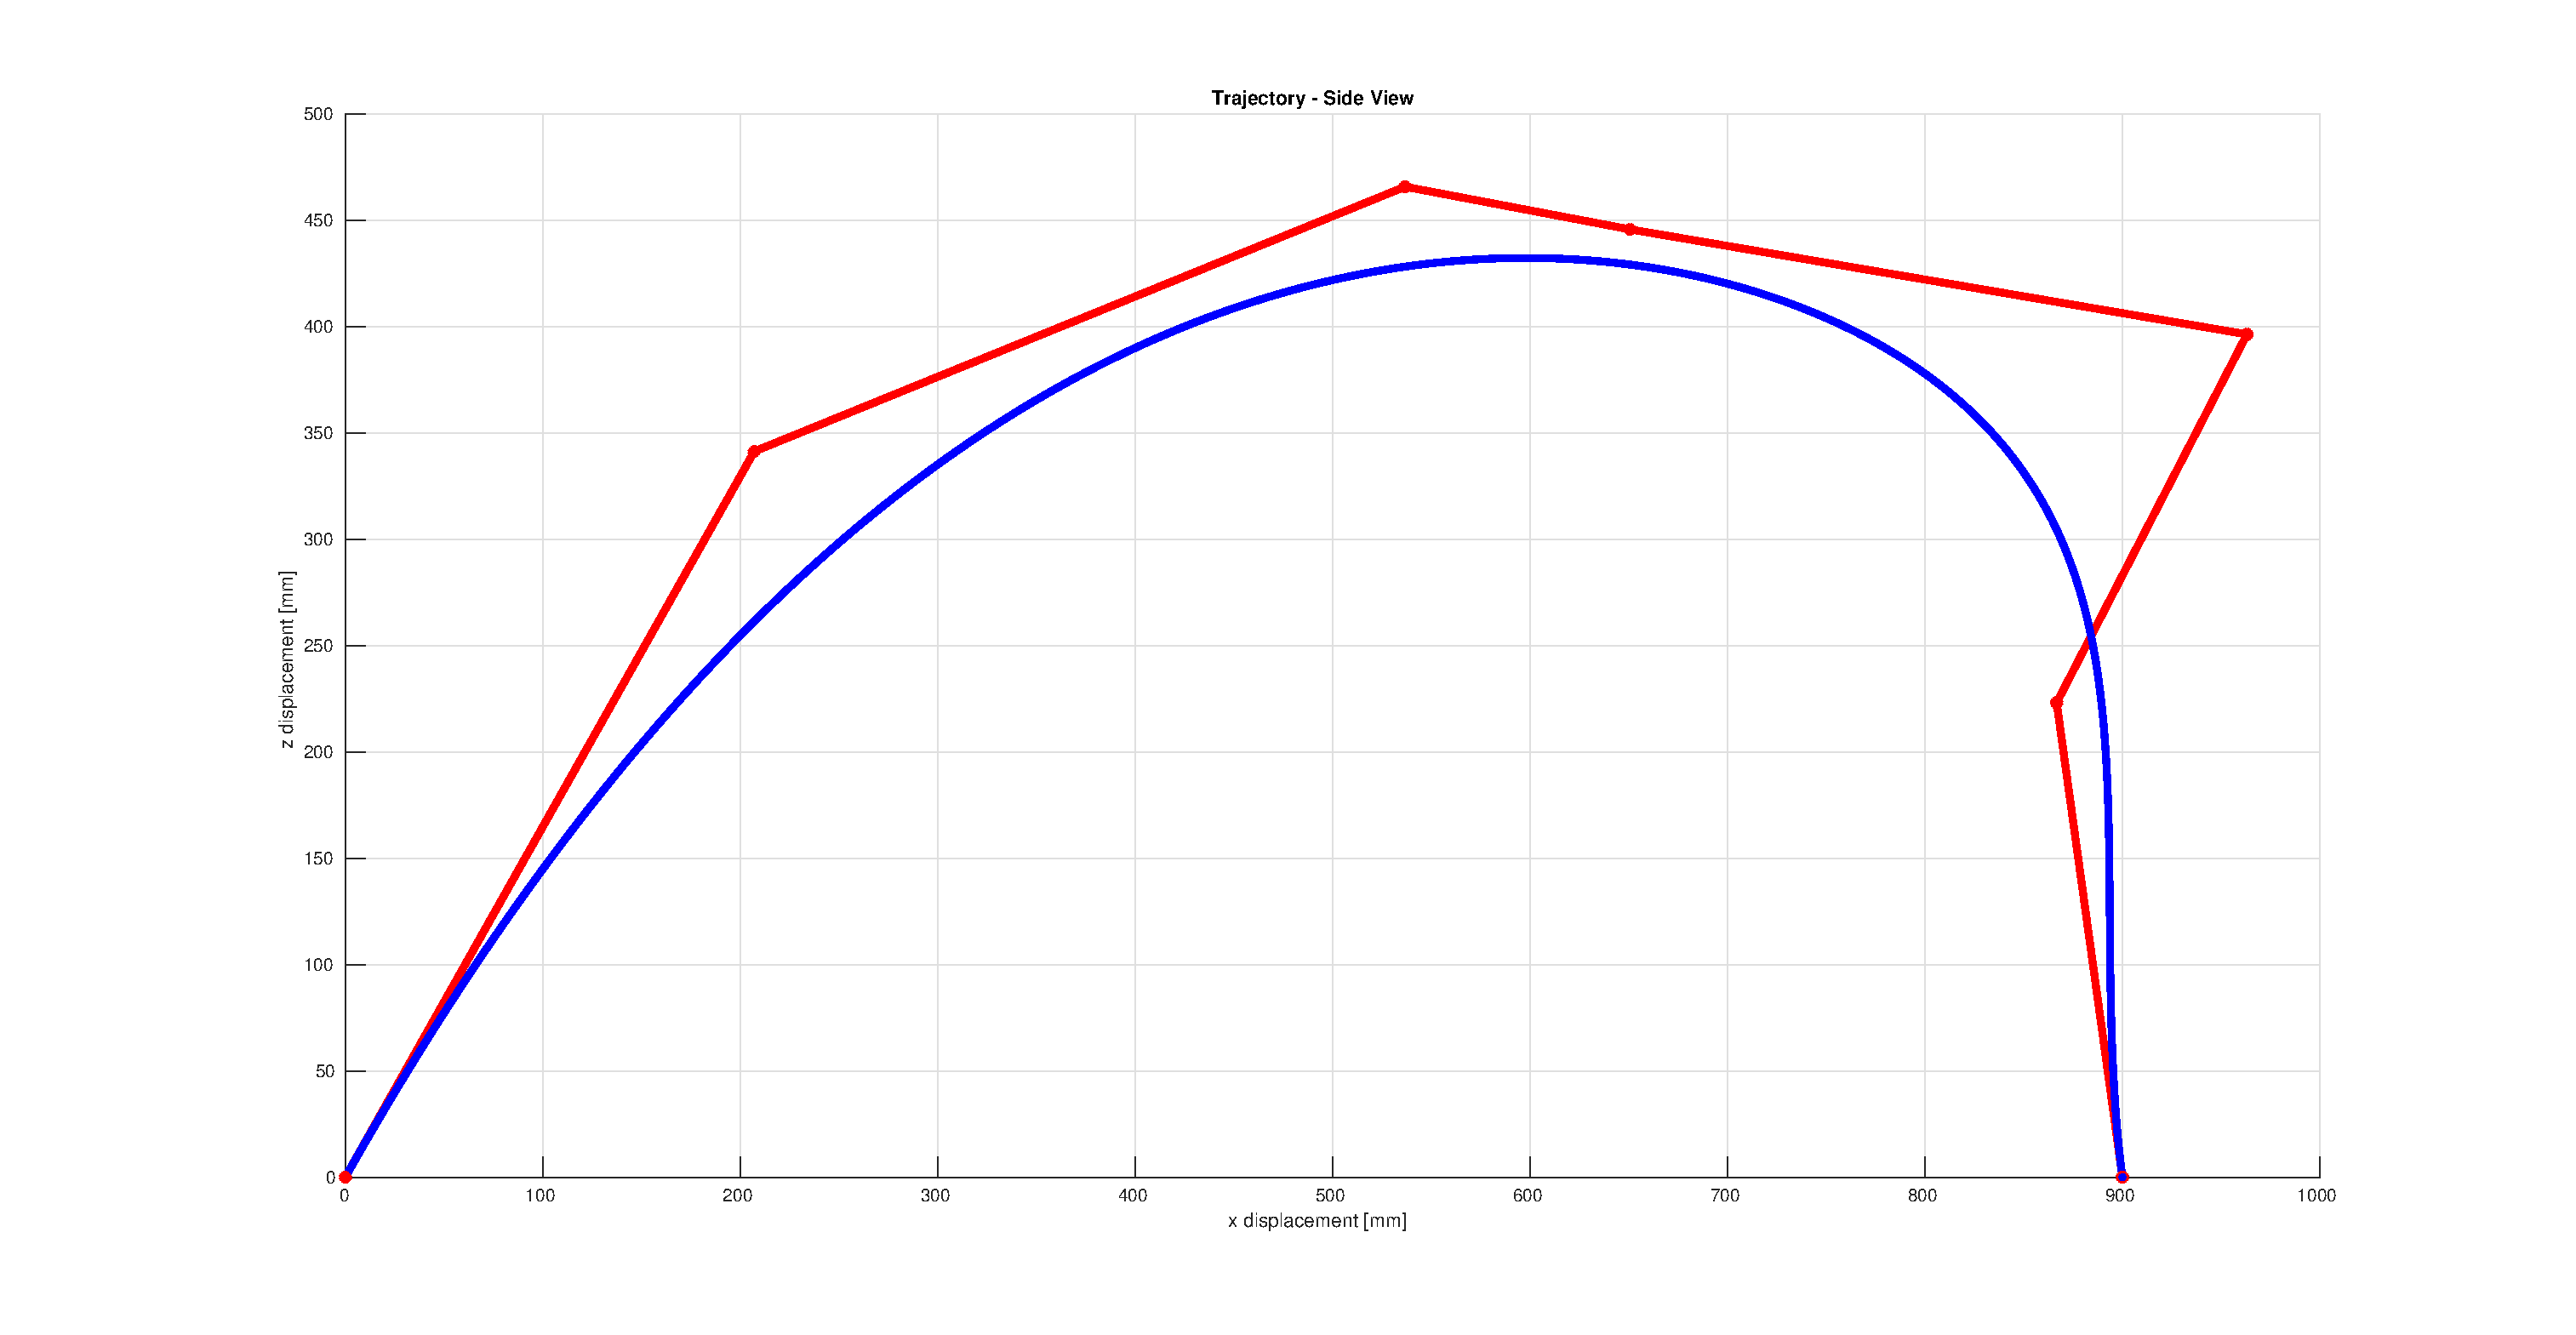
\includegraphics[height=0.45\linewidth, width=0.45\linewidth]{trajectory_simplify_no_subdivide_side.eps}
				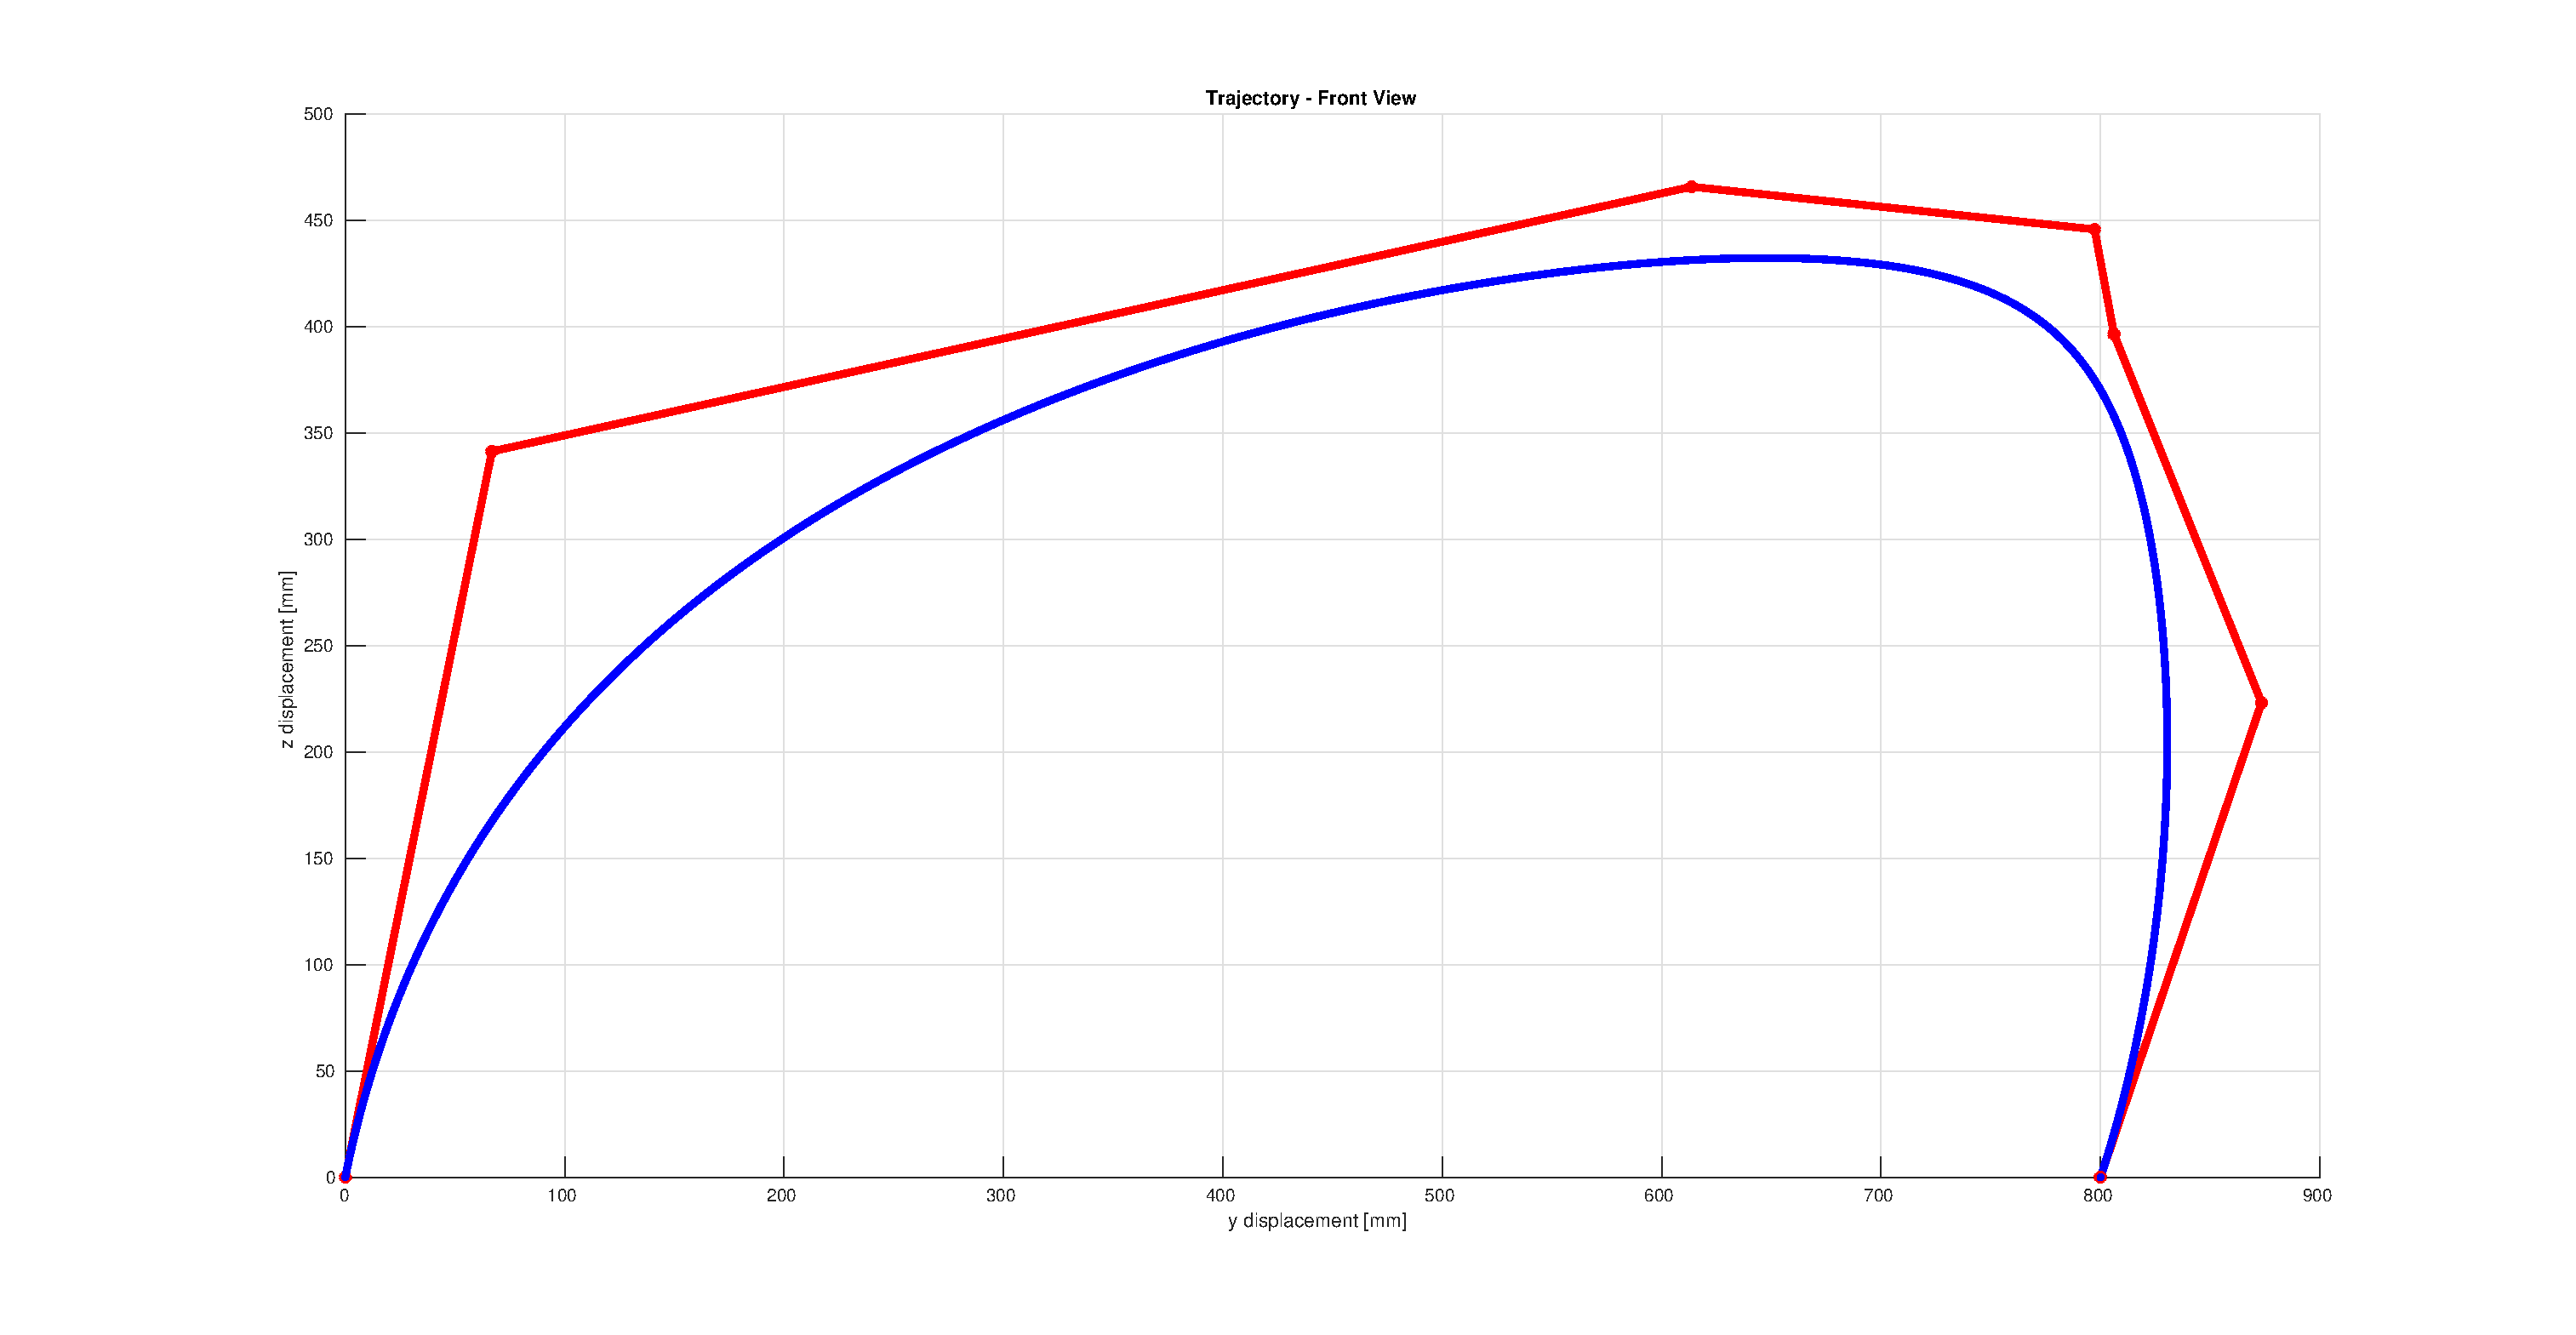
\includegraphics[height=0.45\linewidth, width=0.45\linewidth]{trajectory_simplify_no_subdivide_front.eps}
				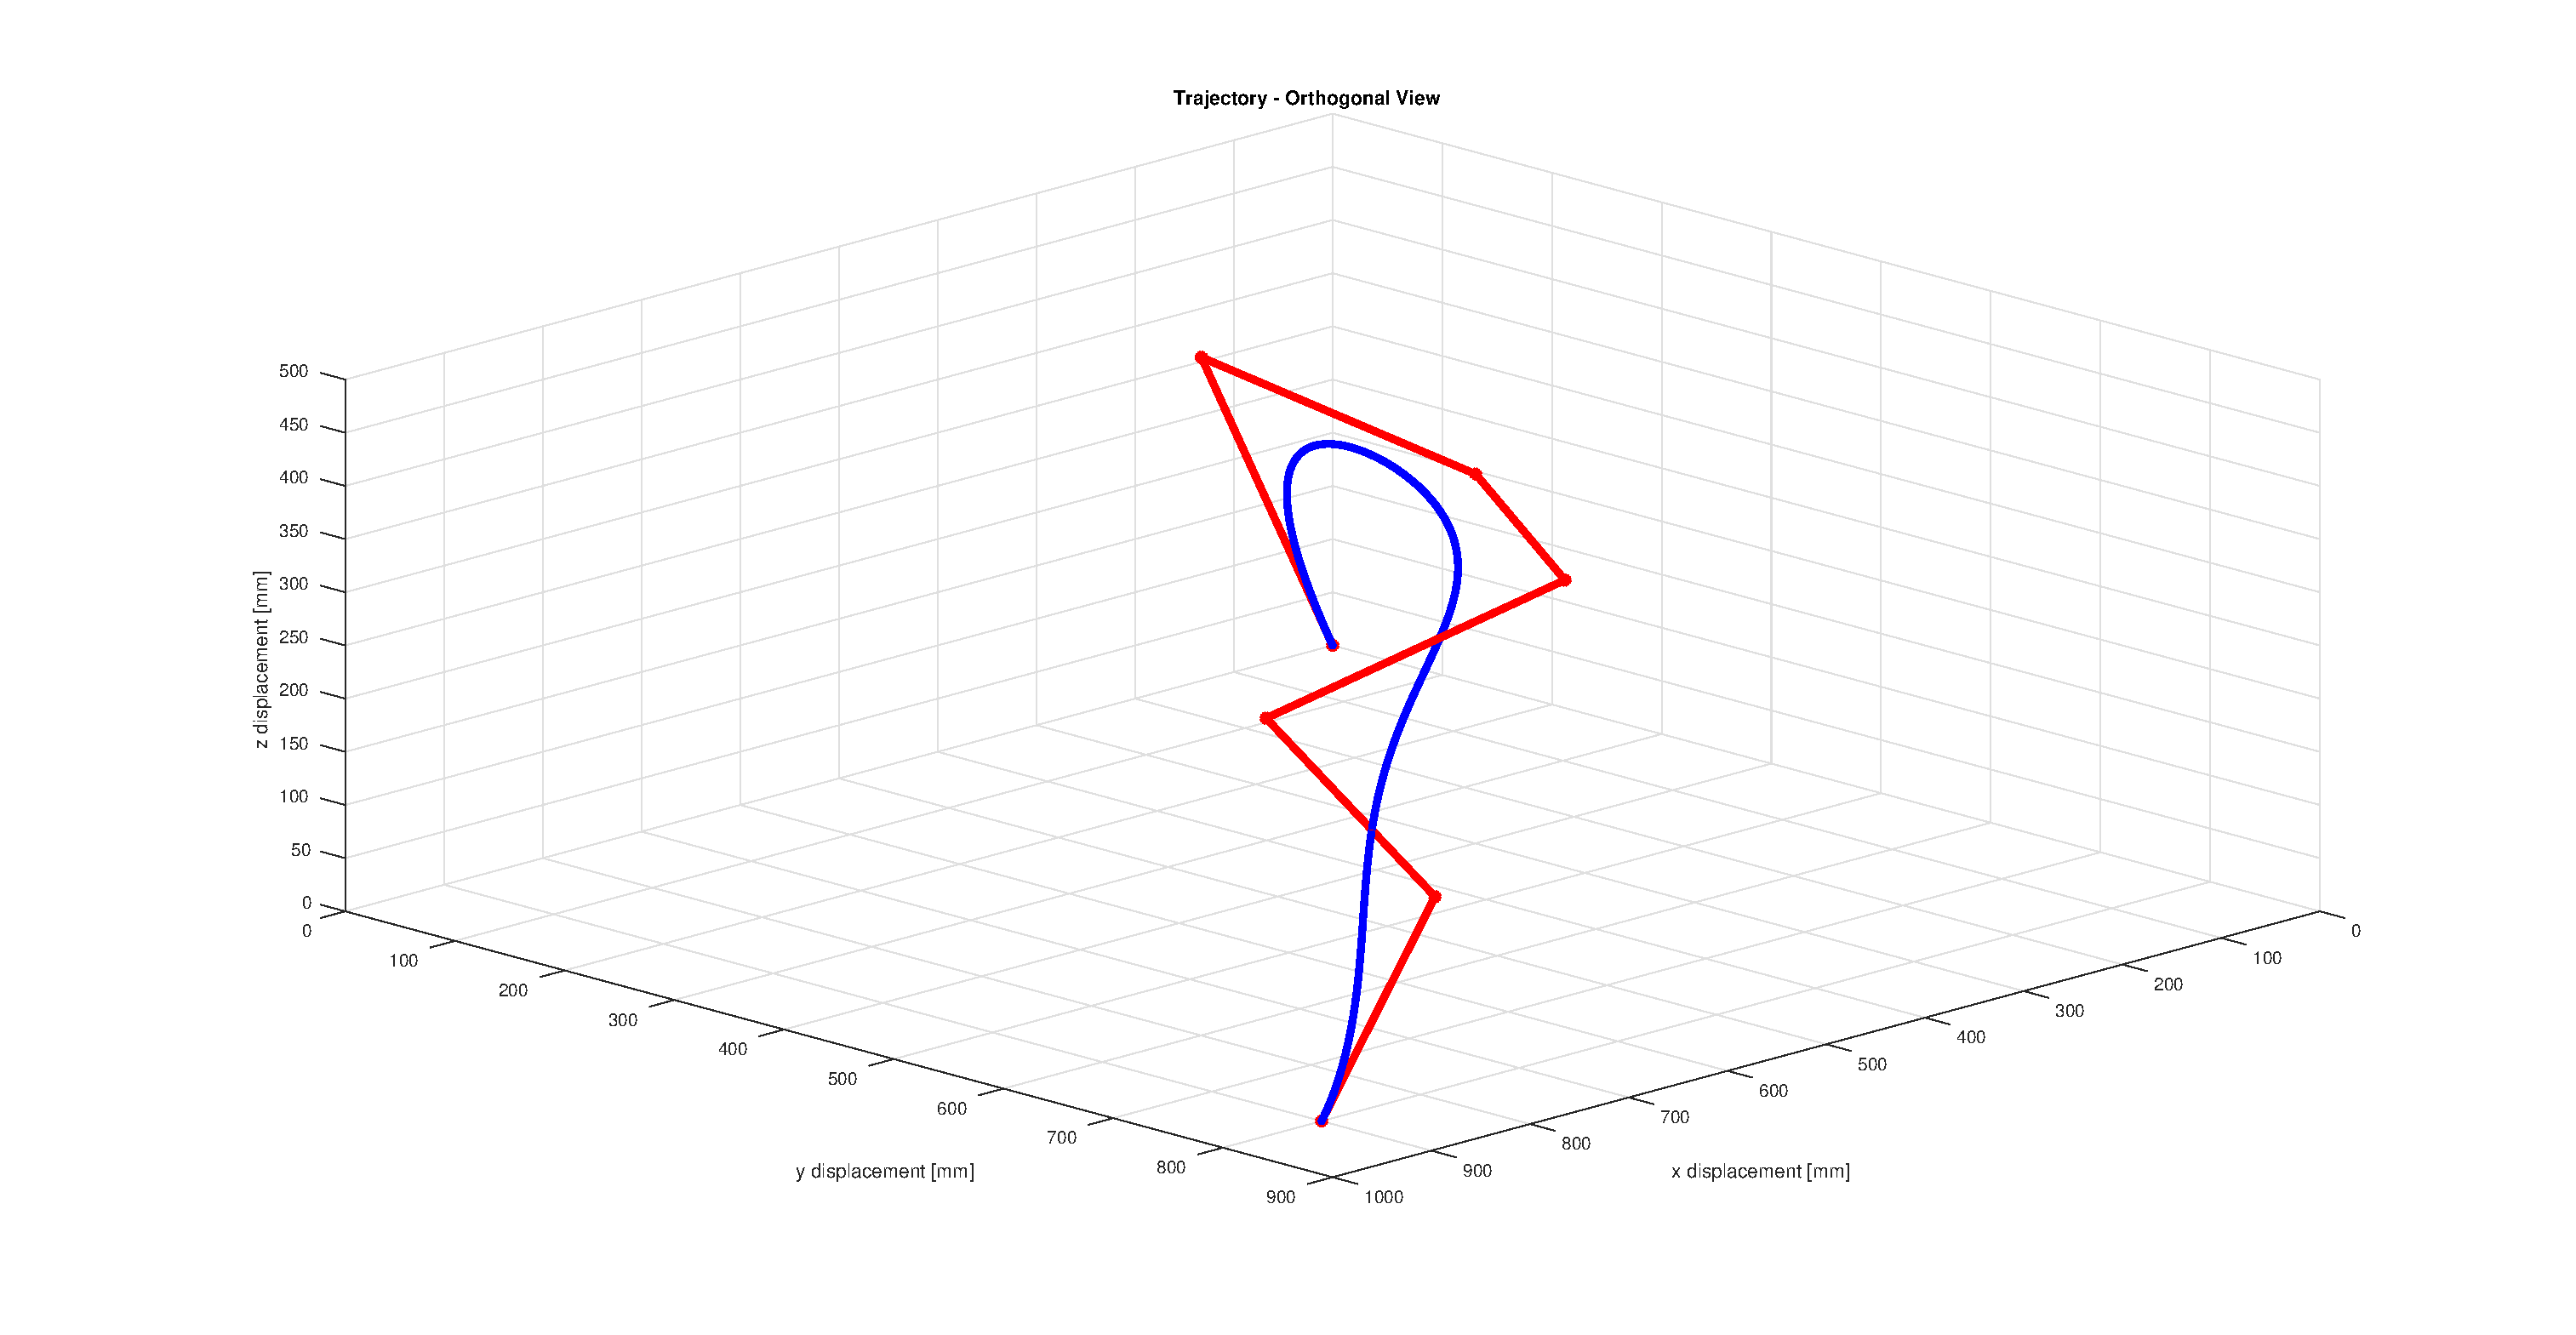
\includegraphics[height=0.45\linewidth, width=0.45\linewidth]{trajectory_simplify_no_subdivide_orthogonal.eps}
				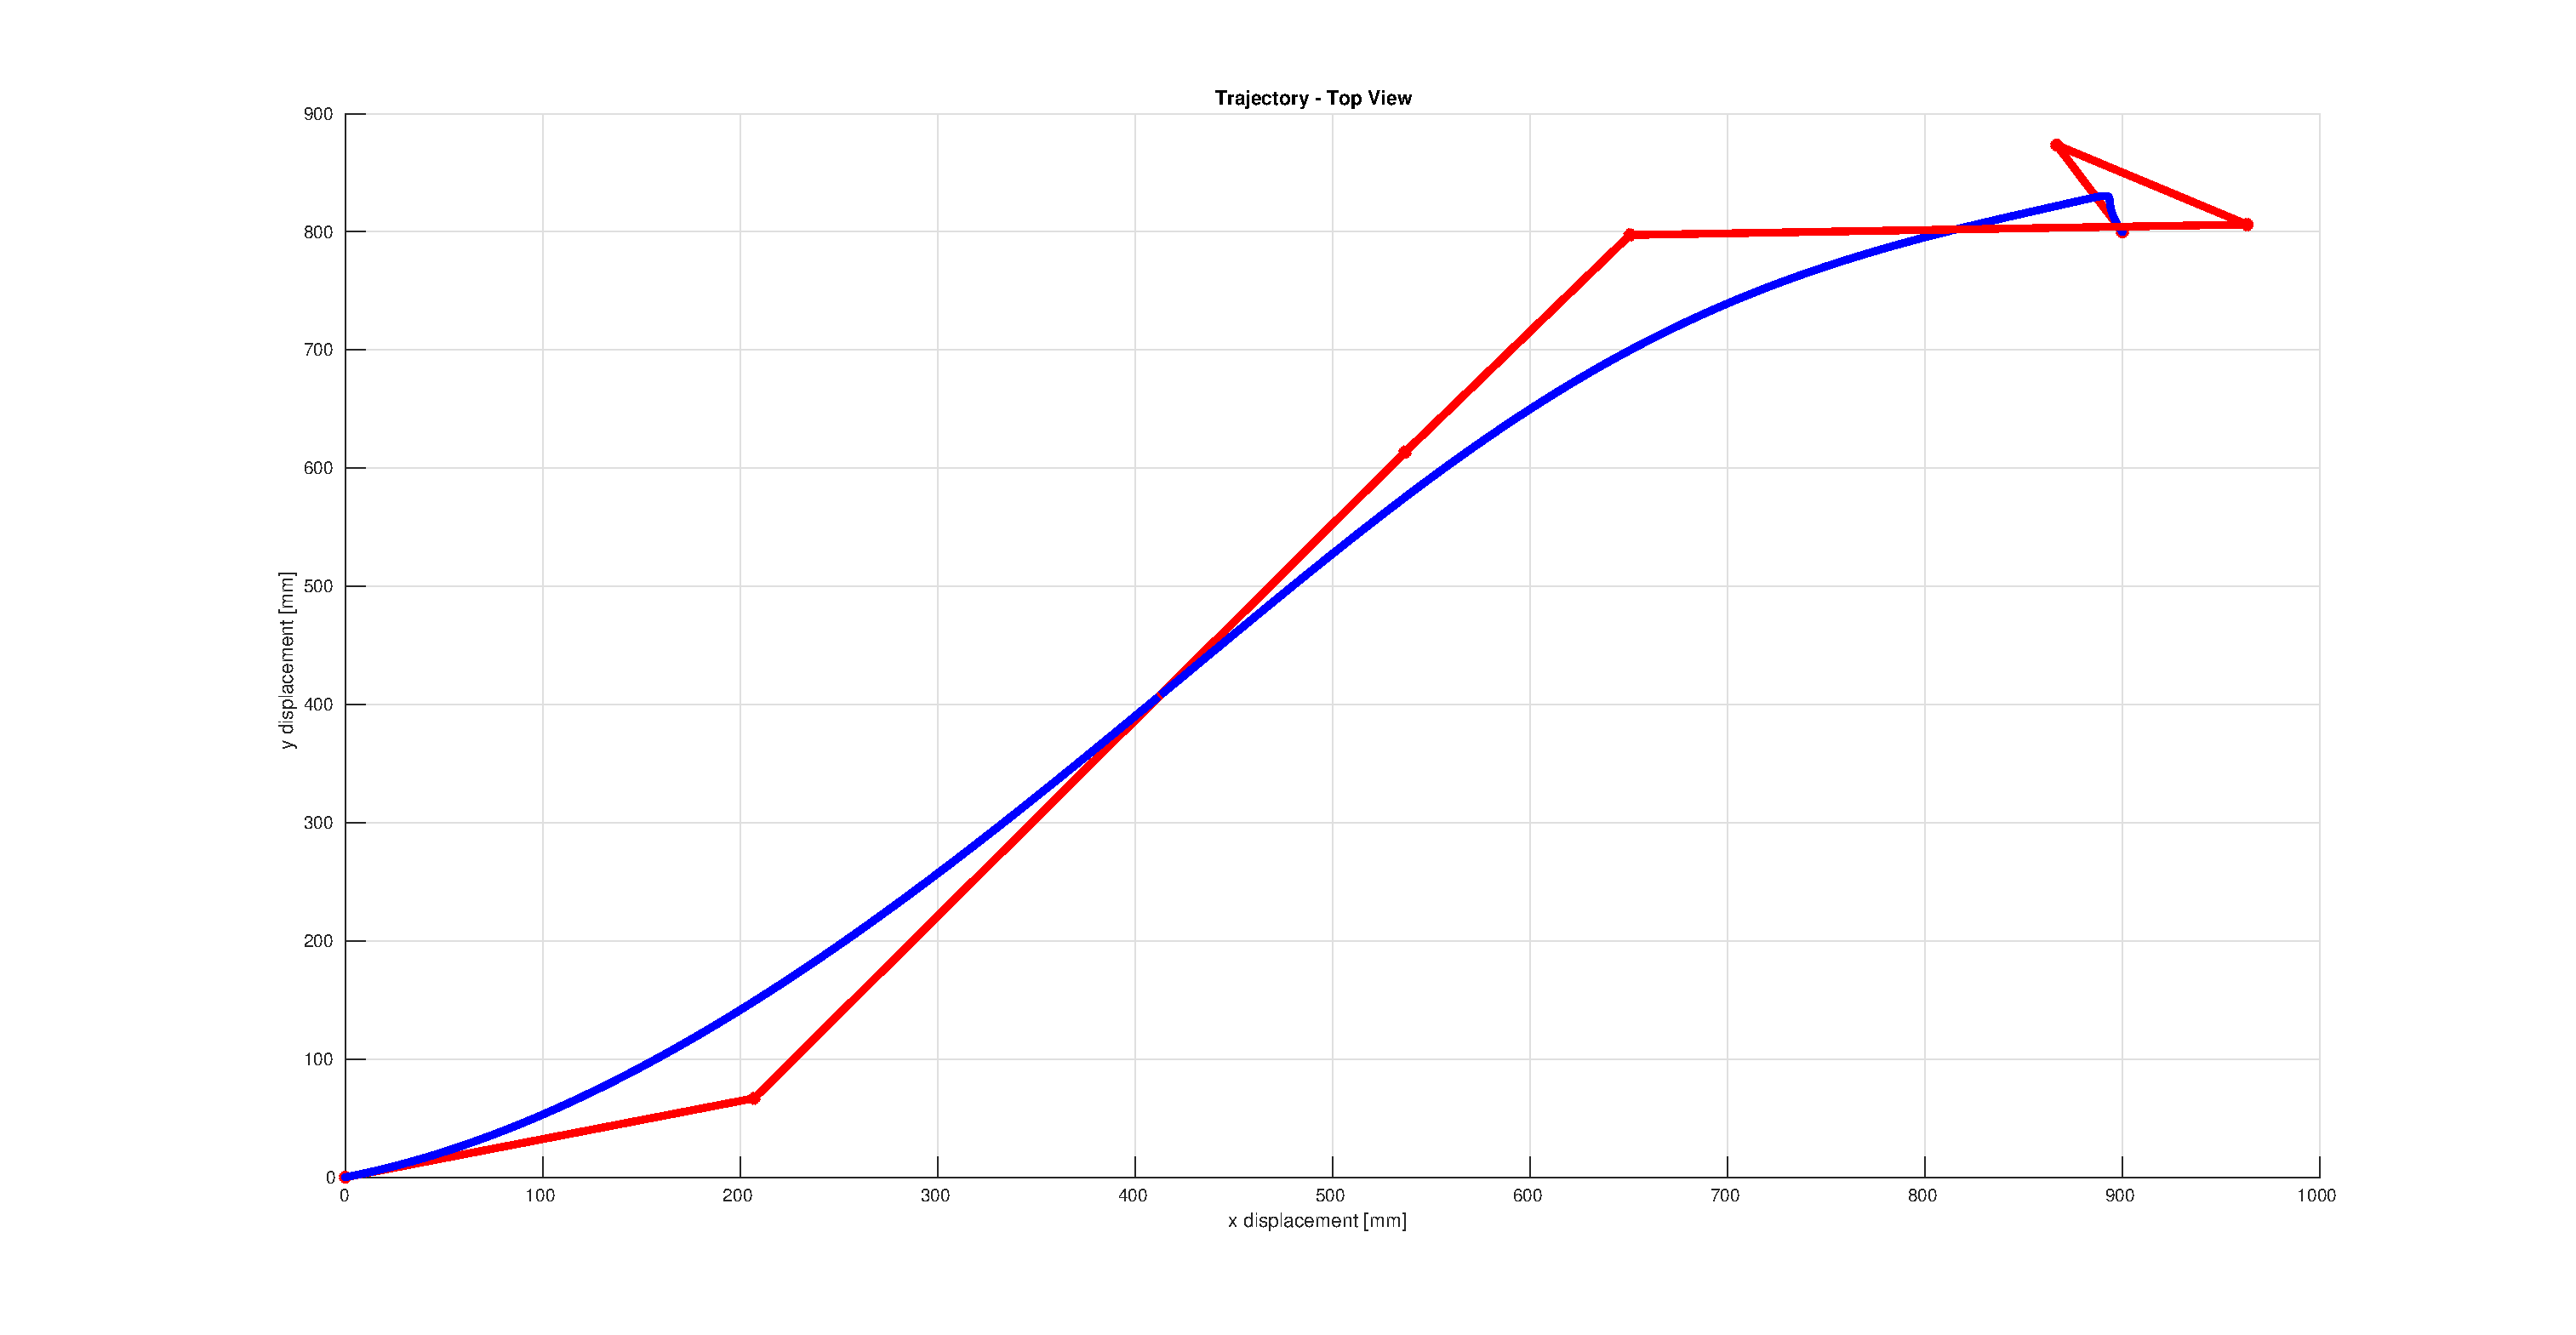
\includegraphics[height=0.45\linewidth, width=0.45\linewidth]{trajectory_simplify_no_subdivide_top.eps}
			\end{minipage}
			\caption{Sample Trajectory without Augmenting $\setofposes$}
			\label{fig:sample_trajectory_after_simplification}
		\end{figure}


		\begin{figure}[hb]
			\centering
			\begin{minipage}{0.8\linewidth}
				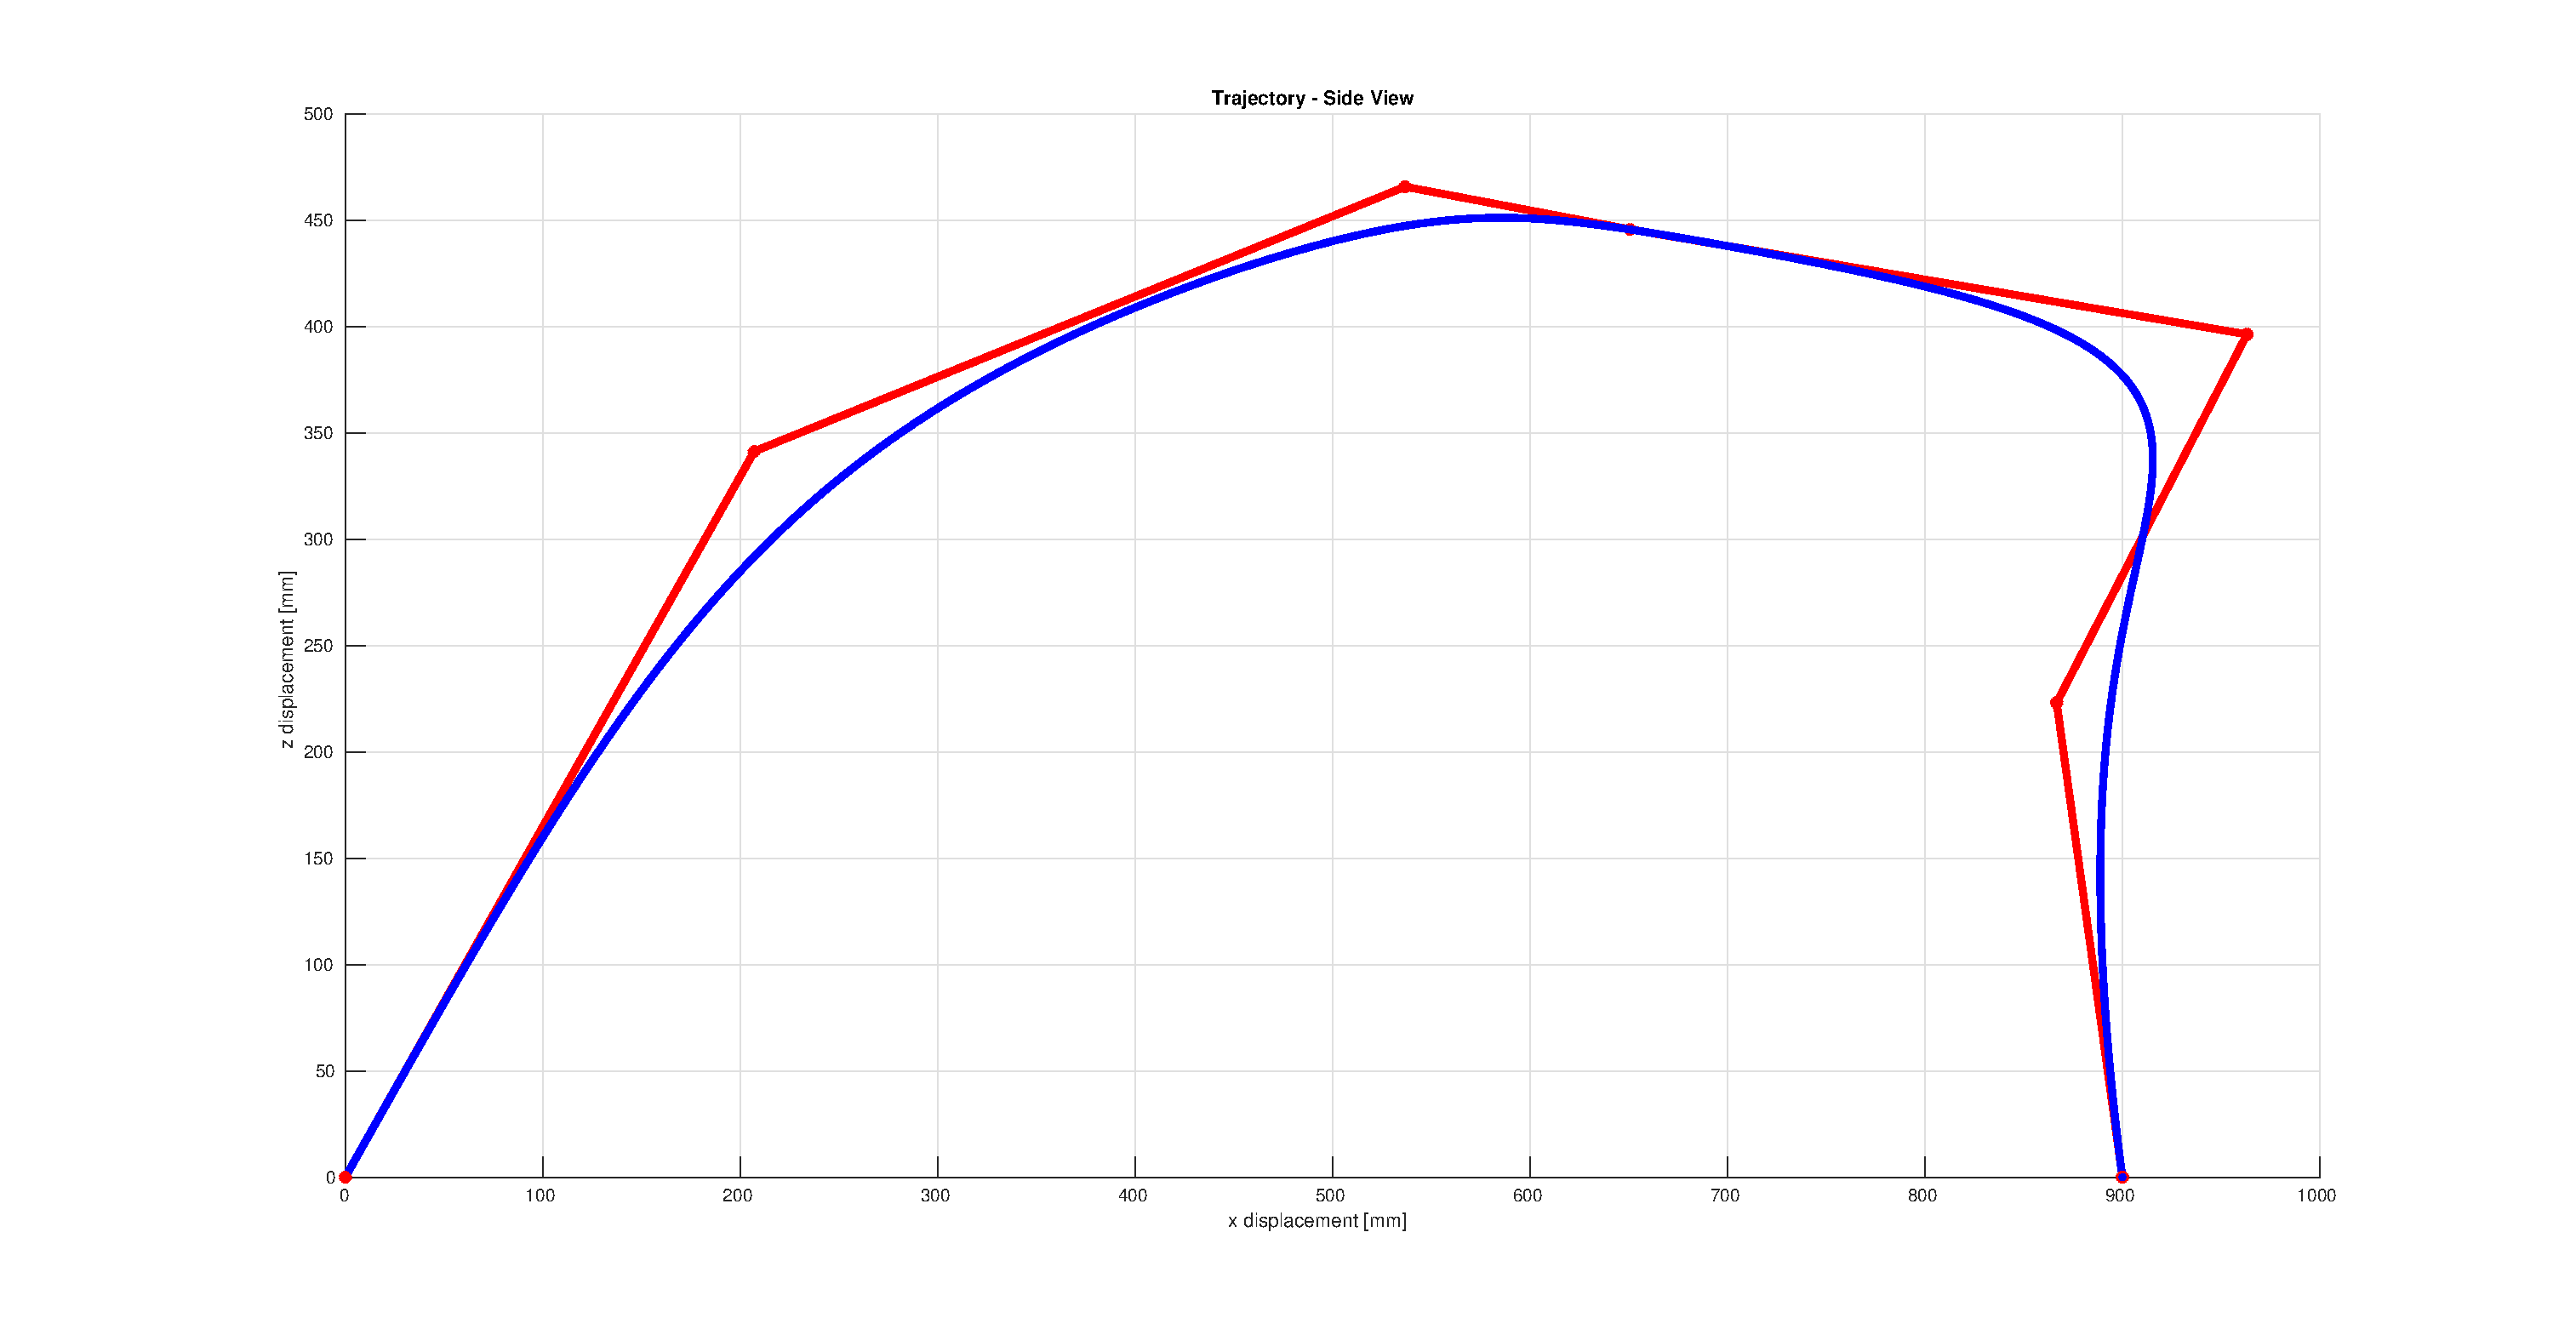
\includegraphics[height=0.45\linewidth, width=0.45\linewidth]{trajectory_simplify_subdivide_side.eps}
				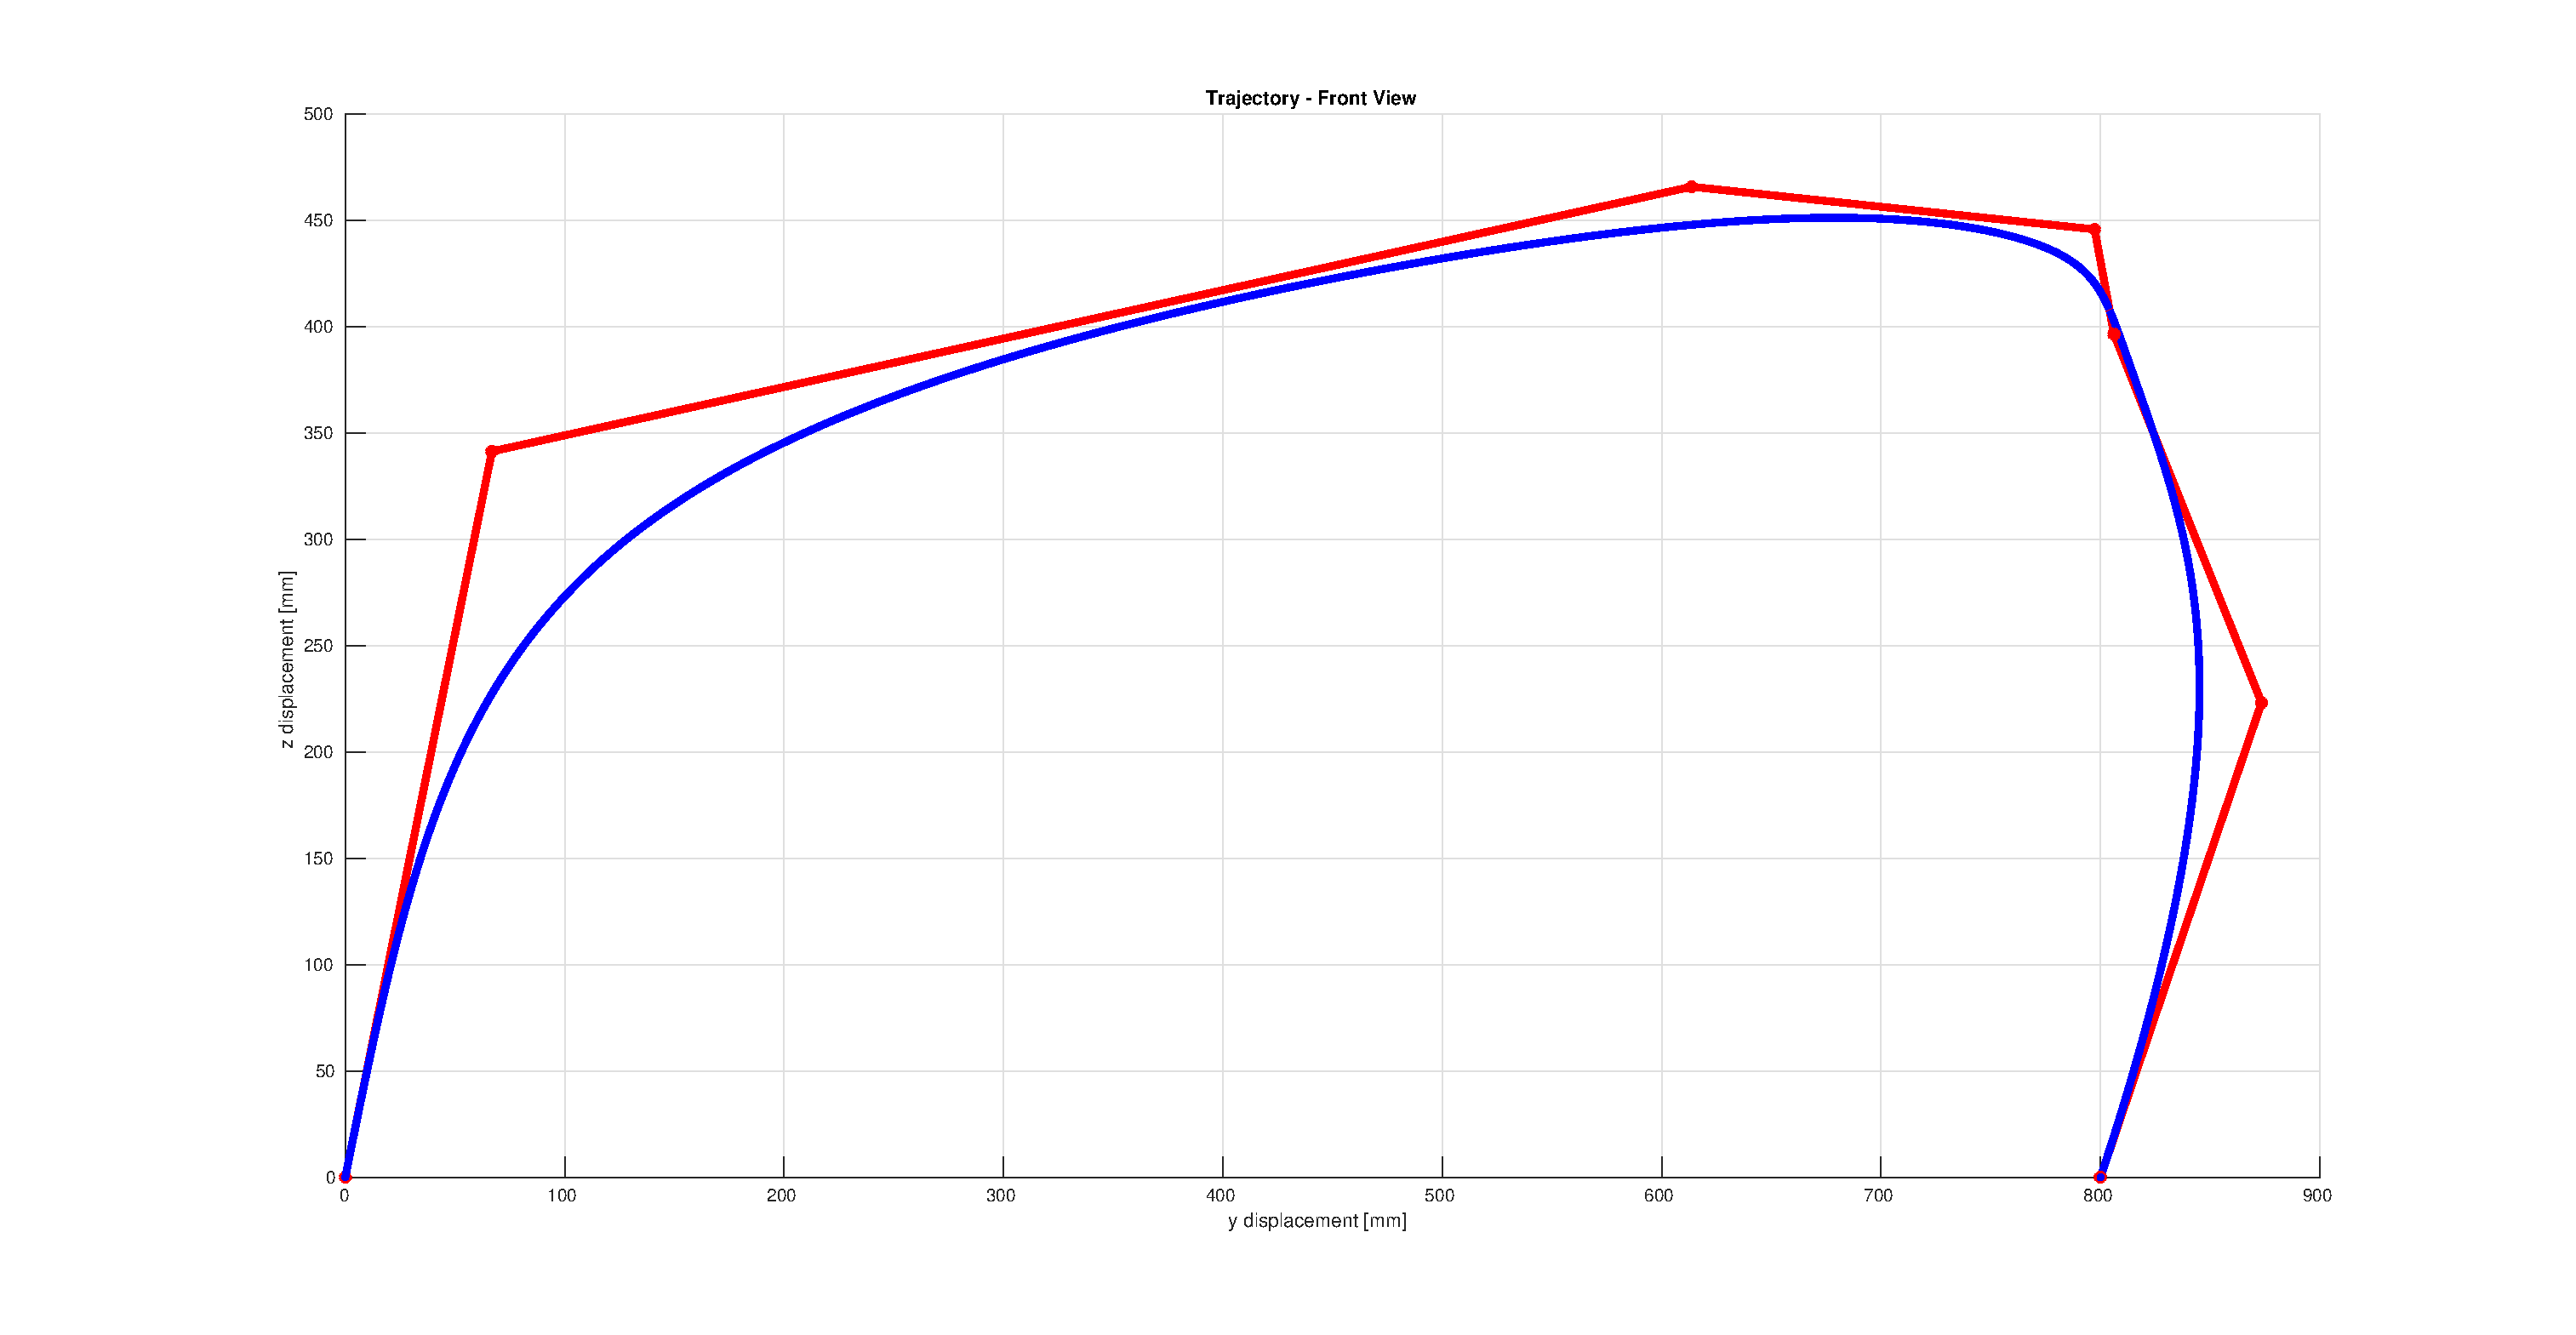
\includegraphics[height=0.45\linewidth, width=0.45\linewidth]{trajectory_simplify_subdivide_front.eps}
				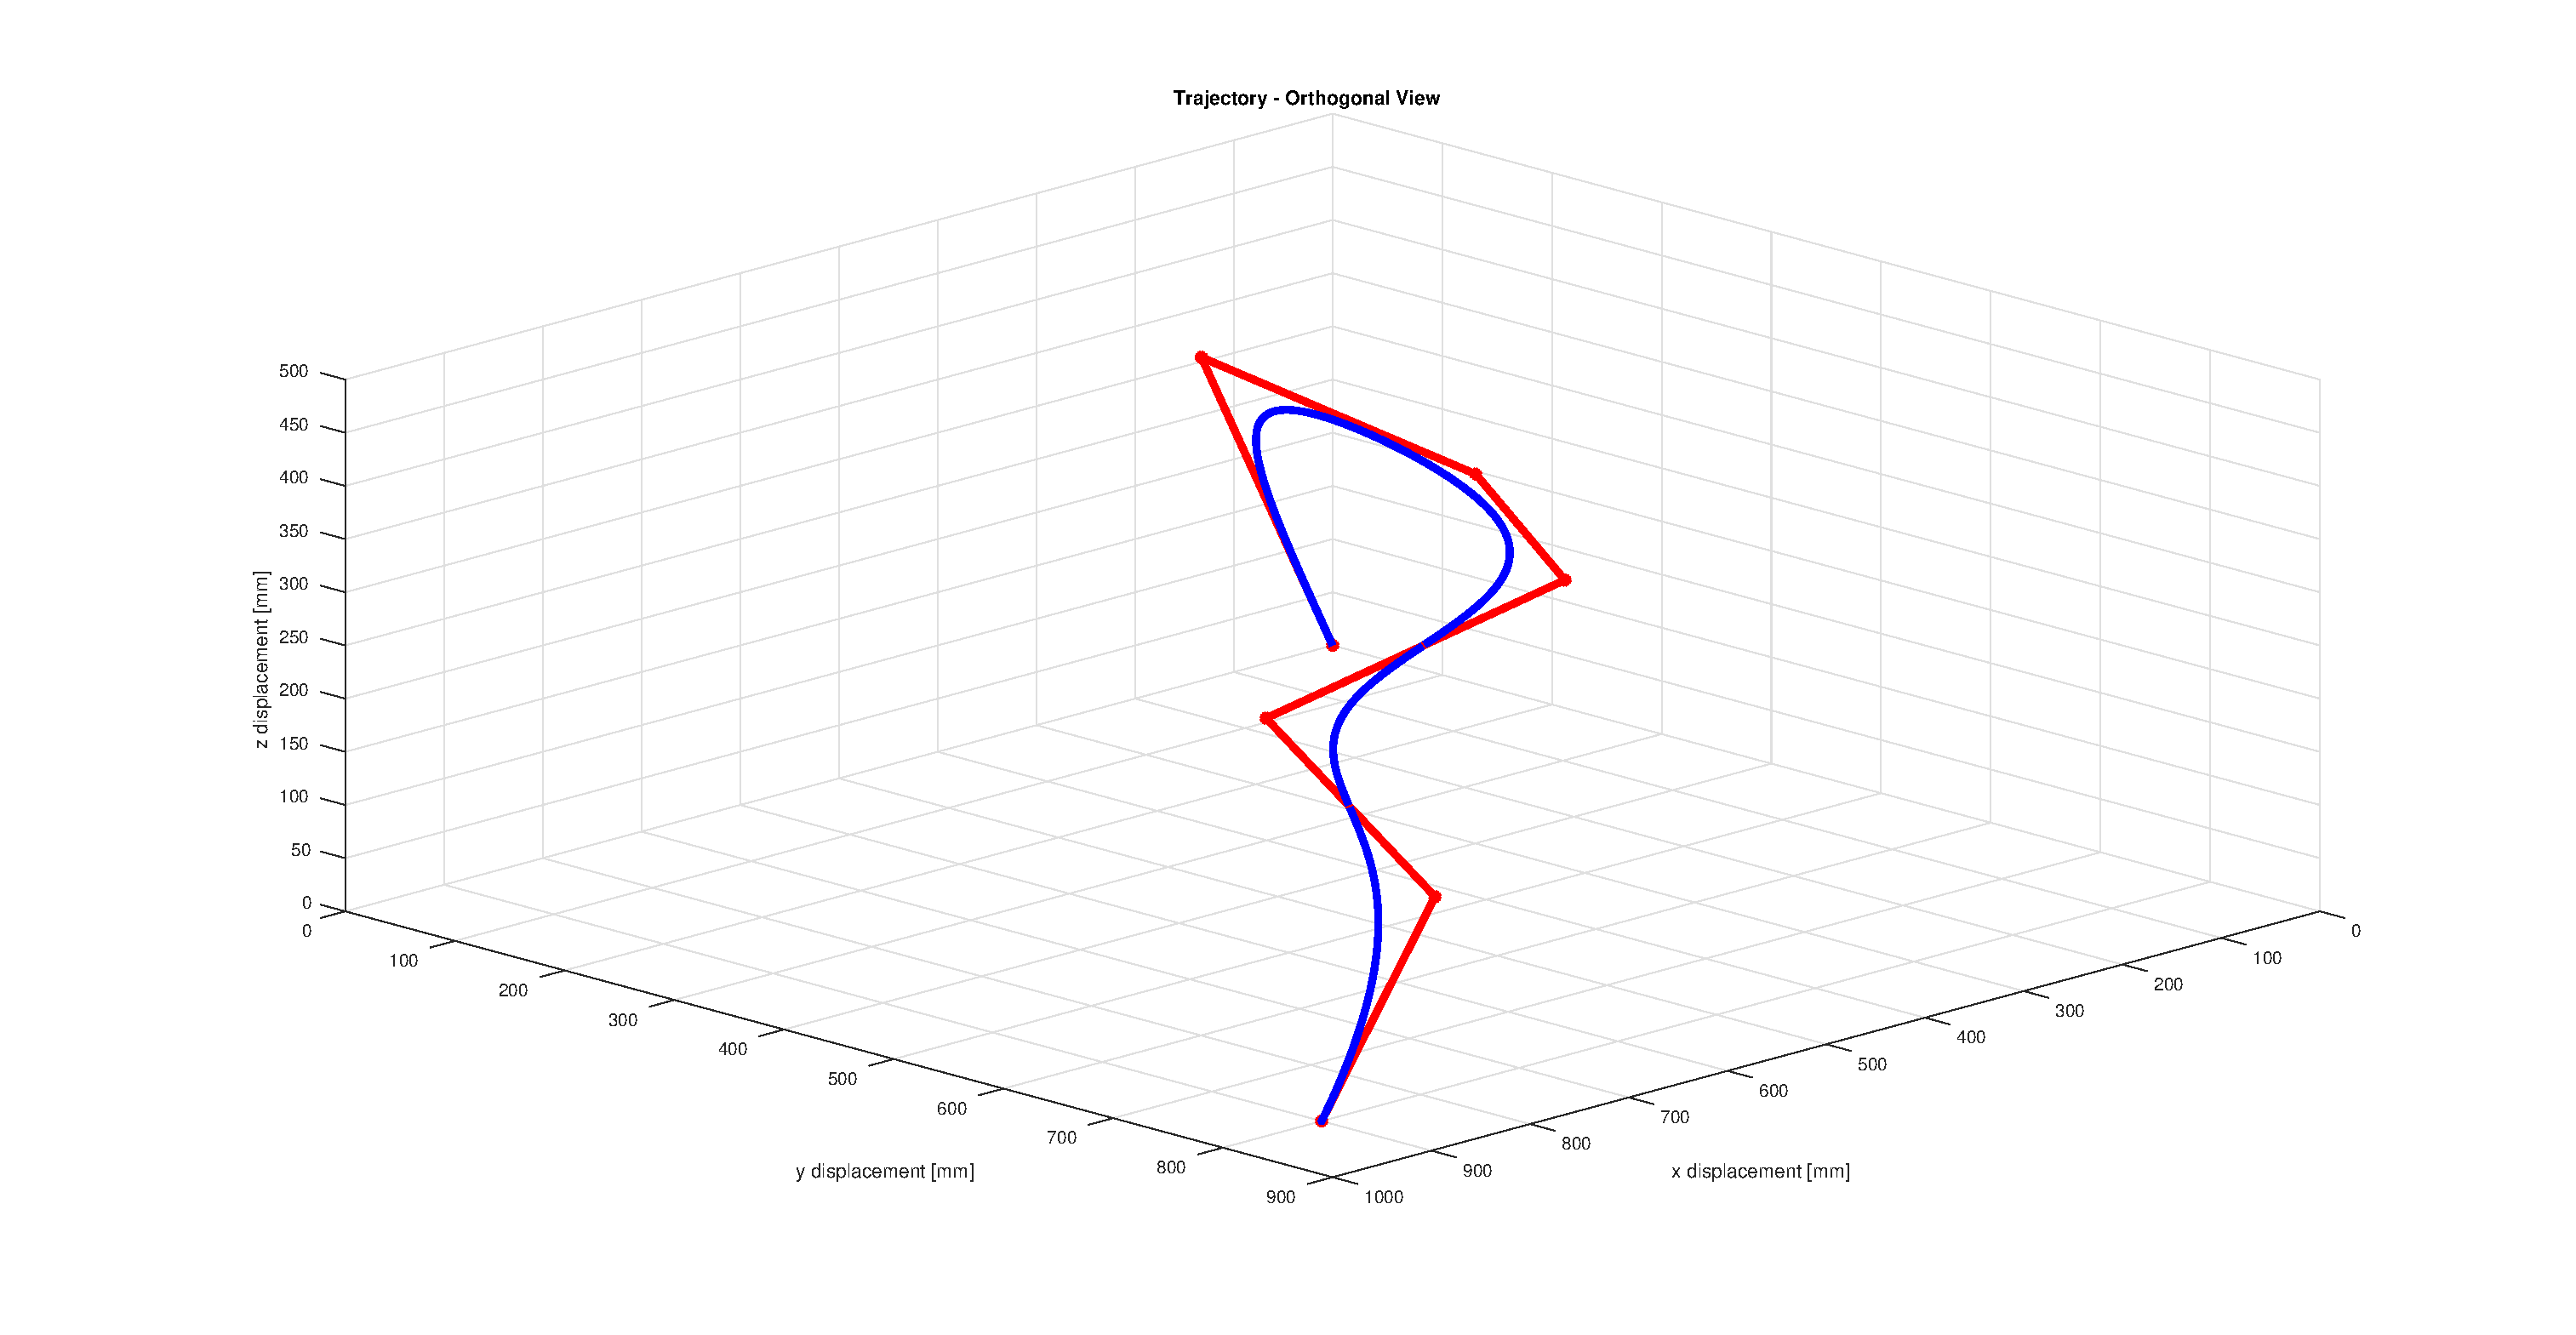
\includegraphics[height=0.45\linewidth, width=0.45\linewidth]{trajectory_simplify_subdivide_orthogonal.eps}
				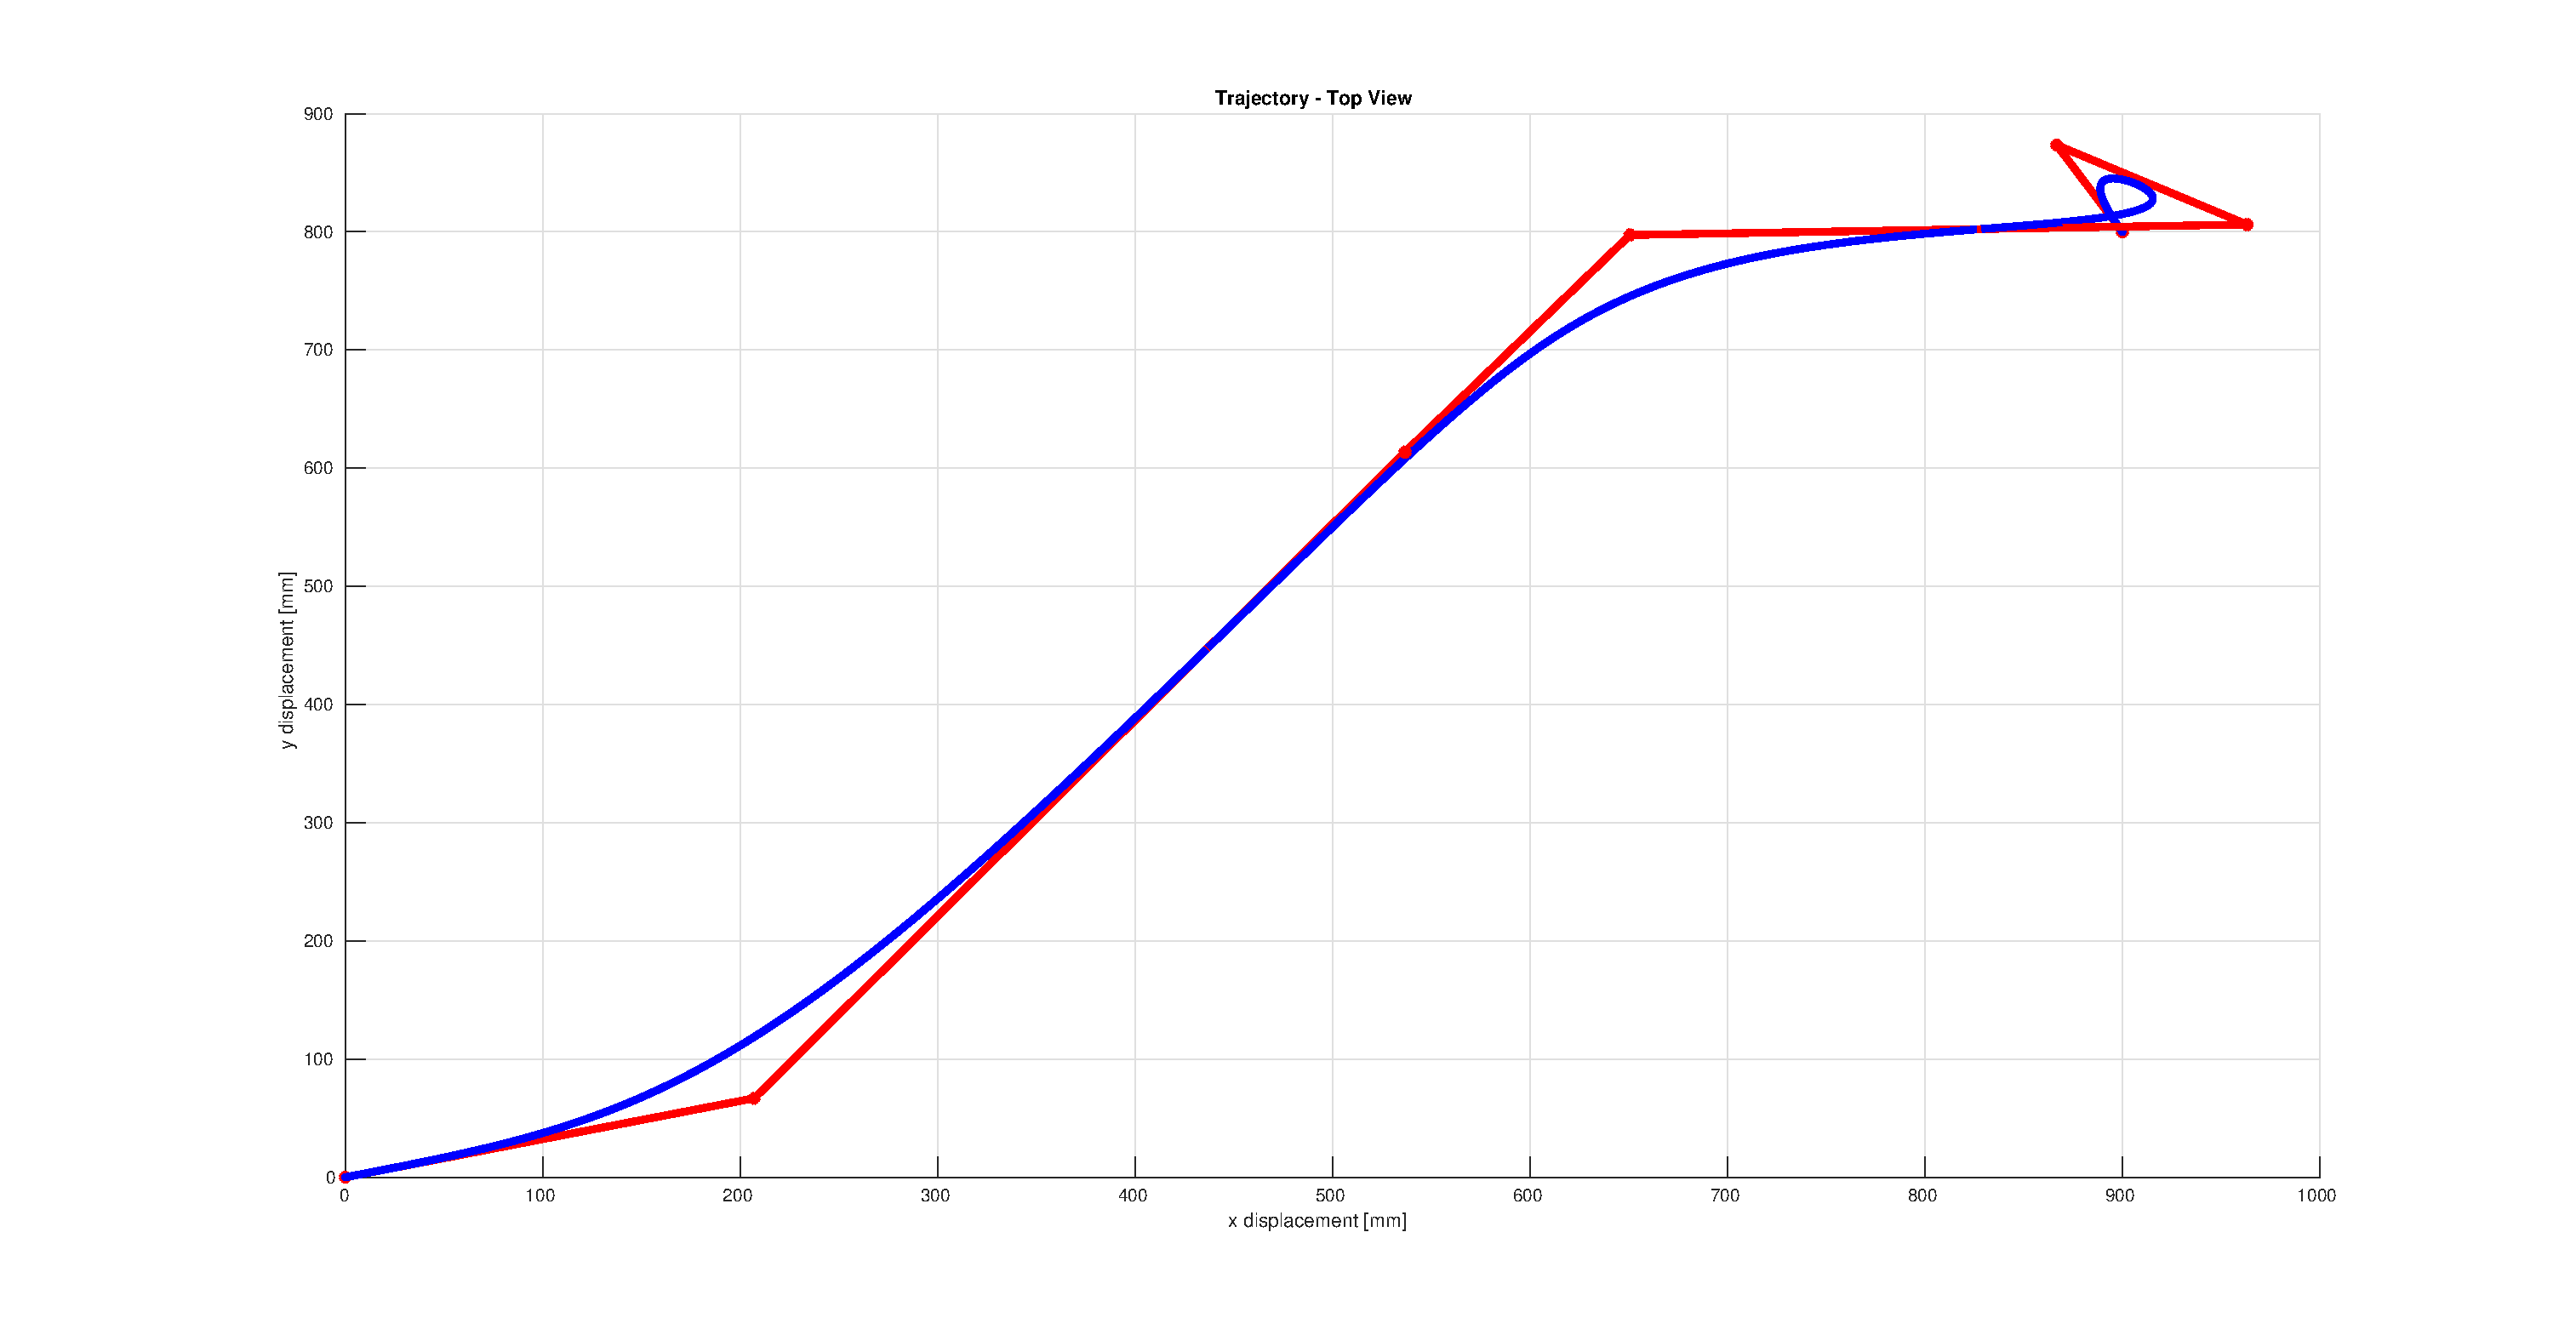
\includegraphics[height=0.45\linewidth, width=0.45\linewidth]{trajectory_simplify_subdivide_top.eps}
			\end{minipage}
			\caption{Sample Trajectory with Augmented $\setofposes$}
			\label{fig:sample_trajectory_with_augmented_set_of_poses}
		\end{figure}
